\documentclass[acmsmall,screen,review,anonymous]{acmart}

\usepackage{booktabs}
\usepackage{tikz}
\usetikzlibrary{arrows.meta,positioning,calc,fit}
\usepackage{pgfplots}
\pgfplotsset{compat=1.17}
\usepackage{listings}
\usepackage{enumitem}

\setcopyright{none}
\acmJournal{PACMPL}
\acmVolume{0}
\acmNumber{PLDI}
\acmYear{2027}

% ---------------------------------------------------------------- macros
% Typography: the calculus is always written "rho calculus", never with the
% Greek letter. Quotation is @P and dereference (drop) is *x.
\newcommand{\quo}[1]{@#1}
\newcommand{\drp}[1]{{*}#1}
\newcommand{\inp}[3]{\mathsf{for}(#1 \leftarrow #2)\,#3}
\newcommand{\out}[2]{#1!(#2)}
\newcommand{\nil}{\mathbf{0}}
\newcommand{\enc}[1]{[\![#1]\!]}
\newcommand{\nameq}{\equiv_{\mathcal{N}}}
\newcommand{\Ctx}{\mathscr{C}}
\newcommand{\bisim}{\approx}
\newcommand{\fn}{\mathrm{fn}}
\newcommand{\red}{\longrightarrow}
\newcommand{\wred}{\longrightarrow^{*}}
\newcommand{\scong}{\equiv}
\newcommand{\mm}{\mathsf{m}}
\newcommand{\dd}{\mathsf{d}}
\newcommand{\kk}{\mathsf{k}}
\newcommand{\fw}{\mathsf{fw}}
\newcommand{\bl}{\mathsf{b}_{\mathsf{l}}}
\newcommand{\br}{\mathsf{b}_{\mathsf{r}}}
\newcommand{\sy}{\mathsf{s}}
\newcommand{\ev}{\mathsf{e}}
\newcommand{\qq}{\mathsf{q}}
\newcommand{\cons}{\mathsf{cons}}
\newcommand{\inst}{\mathsf{inst}}
\newcommand{\hole}{\Box}
\newcommand{\Wt}{\mathrm{wt}}
\newcommand{\tool}{\textsf{f1r3comb}}
\newcommand{\rc}{\textsc{RC}}
\newcommand{\rcnu}{\textsc{RC}^{\nu}}

\AtEndPreamble{\theoremstyle{acmdefinition}\newtheorem{remark}[theorem]{Remark}}

\begin{document}

\title{Compiling the Rho Calculus to Data-Parallel Hardware through Name-Free Combinators}

\author{Anonymous Author(s)}
\affiliation{\institution{Anonymous Institution}\country{Anonymous}}

\begin{abstract}
Process calculi with mobile names are a natural description of concurrent
systems and a poor fit for graphics processors. An interpreter for such a
calculus matches patterns modulo structural congruence, manages binders, and
chases pointers through a store of variably shaped terms; a GPU wants flat
arrays of fixed-width records, uniform work across lanes, and bulk-synchronous
phases built from sort, scan and join. We close this gap for the rho calculus,
a reflective higher-order process calculus in which names are quoted
processes, by compiling it into a calculus of \emph{name-free combinators}
whose states are multisets of fixed-width tuples of integers.

The compiler runs in two phases. Phase one eliminates the input binder by
reflection: a continuation is quoted once and released by a three-atom gate,
so the image is linear in the source, where the classical combinator
elimination of the asynchronous $\pi$-calculus is exponential in nesting
depth. Phase two eliminates the auxiliary name binder by running each
instance of compiled code at a run-time \emph{address}. We show that the
obvious way to do this, erecting apparatus with fixed-arity name
constructors, is unsound on a bulk-synchronous machine: concurrently erected
instances mix their apparatus in up to all runs. We prove that no fixed-arity
construction satisfies the discipline that prevents mixing, and that a
single-premise \emph{context-instantiation} combinator does, erecting any
instance in two steps. The translation is fully abstract relative to encoded
contexts.

On the target, structural congruence is free, pattern matching has moved into
the compiler, redex finding is a relational join on a term-sized incidence
matrix, and a machine step is a maximal independent set of redexes, which we
prove sound with respect to interleaving semantics. We implement the compiler
and the machine in Rust with WGSL kernels generated from the rule table, and
evaluate on program families whose parallel structure is known. Machine steps
track causal depth rather than work: parallel steps stay constant as width
grows 64-fold, and a balanced distributor, a one-line change to phase one,
reduces the depth of a higher-order benchmark from 266 steps to 20.
\end{abstract}

\begin{CCSXML}
<ccs2012>
<concept><concept_id>10011007.10011006.10011041</concept_id><concept_desc>Software and its engineering~Compilers</concept_desc><concept_significance>500</concept_significance></concept>
<concept><concept_id>10003752.10003753.10003761.10003764</concept_id><concept_desc>Theory of computation~Process calculi</concept_desc><concept_significance>500</concept_significance></concept>
<concept><concept_id>10010147.10010169.10010170</concept_id><concept_desc>Computing methodologies~Parallel algorithms</concept_desc><concept_significance>300</concept_significance></concept>
</ccs2012>
\end{CCSXML}
\ccsdesc[500]{Software and its engineering~Compilers}
\ccsdesc[500]{Theory of computation~Process calculi}
\ccsdesc[300]{Computing methodologies~Parallel algorithms}

\keywords{rho calculus, process calculi, combinators, compilation, GPU,
bulk-synchronous parallelism, multiset rewriting, full abstraction}

\maketitle

% ======================================================================
\section{Introduction}
\label{sec:intro}

Graphics processors are the most widely deployed parallel machines, and the
programming models they reward are narrow. A GPU does well when state is a
flat array of fixed-width records, when neighbouring lanes execute the same
instructions, and when computation proceeds in bulk-synchronous phases
separated by barriers, each phase built from primitives with mature parallel
implementations: sort, prefix scan, hash join, sparse matrix
product~\cite{Valiant90,Blelloch96,GraphBLAS11}. Programs that can be
expressed in these terms inherit decades of tuning. Programs that cannot
mostly do not run on GPUs at all.

Concurrent programs written against mobile process calculi are, on their
face, in the second class. An interpreter for the $\pi$-calculus or one of
its relatives stores a soup of terms of varying shape, reached by pointer. It
finds a communication by matching an input against an output modulo
structural congruence, and it substitutes under binders, which requires
fresh-name management. It resolves competition between redexes by locking or
by a central scheduler. Each of these is expensive on a GPU, and together
they make the calculus look like the wrong starting point.

This paper argues that it is the right starting point, provided one compiles
far enough before running. We take the \emph{rho calculus}~\cite{MeredithRadestock05},
a reflective higher-order process calculus in which every name is the
quotation $\quo{P}$ of a process and every process can be recovered from its
quotation by the drop $\drp{x}$, and compile it into a calculus of
\emph{name-free combinators}: a small, fixed family of atoms, each a head
symbol applied to a bounded number of names, with no binders and no pattern
variables. The target has four properties that match the four demands of
the hardware exactly.
\begin{enumerate}[leftmargin=2em]
\item \emph{States are multisets of fixed-width integer tuples.} Every atom is
  a head symbol and at most four names, names are interned to integers, and
  structural congruence of the target is multiset equality, so it costs
  nothing at run time.
\item \emph{Rules are generated and uniform.} There are twenty rules, all
  generated from a table of twenty-one atom shapes. Each rule is a join of
  one consumer atom against one to three message atoms on shared names, with
  no nested matching.
\item \emph{A step is a bulk operation.} Redex finding for every rule is a
  relational join on an atom--name incidence matrix whose size is that of
  the term, conflict detection is a second product, and a machine step fires
  a maximal independent set of redexes. We prove that firing an independent
  set is sound with respect to interleaving semantics, so the number of
  machine steps is bounded by the causal depth of the computation rather
  than its length.
\item \emph{Reflection becomes an intern table.} The feature that makes the
  source calculus theoretically demanding --- that a name is a program --- is,
  on the machine, a bidirectional hash-consing table. Opening a quoted
  continuation is a table read followed by a contiguous copy, and building a
  name is an insert-or-get.
\end{enumerate}

The compiler that produces such terms is the technical heart of the paper,
and it turns out to be more delicate than its sequential predecessors suggest.

\paragraph{Binders by reflection.}
\citet{Yoshida02} showed that the input binder of the asynchronous
$\pi$-calculus can be eliminated in favour of combinators, keeping
name restriction. Her elimination pushes each prefix through its body,
splitting at every parallel composition, so the image of a nesting of $d$
inputs has $\Theta(3^{d})$ atoms. In the rho calculus a continuation can
instead be \emph{quoted once} and stored behind a three-atom gate that
releases it when the input fires. The image is linear in the source
(\S\ref{sec:phase1}). This is the same move as supercombinator
compilation~\cite{Hughes82} made in a concurrent setting, and it is where
reflection first pays for itself.

\paragraph{Freshness at run time, and a race that breaks it.}
Phase one leaves a name binder, $\mathsf{new}$, around the apparatus of each
compiled input, and phase two must remove it. Allocating apparatus names by
syntactic position is unsound as soon as compiled code is instantiated
twice, which higher-order programs do routinely (\S\ref{sec:positional}). The
fix is to allocate apparatus at run time beneath an \emph{address} each
instance receives. But erecting an atom at allocated names on a
bulk-synchronous machine is itself a join, and joins at shared channels can
draw their inputs from different instances. We measure the consequence ---
concurrent erection by fixed-arity name constructors mixes the apparatus of
distinct instances in 29 of 50 runs with two instances and all 50 runs with
eight --- and prove it is unavoidable for that construction
(Proposition~\ref{prop:multiplicity}). A single combinator that instantiates
a whole context from one address, in one step with one premise, meets the
discipline by construction and erects any instance in two machine steps
(\S\ref{sec:phase2}).

\paragraph{Contributions.}
\begin{itemize}[leftmargin=1.5em]
\item A repaired name-free combinator calculus for the rho calculus, fit to
  serve as a data-parallel intermediate representation. We identify the
  defect that made the published calculus unsound, add the name
  constructors without which no encoding of the rho calculus exists, and
  add the context-instantiation combinator $\inst$ (\S\ref{sec:target}).
\item A two-phase compiler from the rho calculus to these combinators,
  linear in the size of its input, with a proof that the translation is
  fully abstract relative to encoded contexts and that the relativisation
  is forced (\S\ref{sec:compile}).
\item An analysis of instance mixing under concurrent erection: a
  discipline that excludes it, a proof that fixed-arity constructors cannot
  meet the discipline, and a single-premise primitive that does
  (\S\ref{sec:phase2}).
\item A bulk-synchronous abstract machine whose step is a maximal
  independent set of redexes found by joins, with a soundness theorem, and
  an account of how the expressiveness lattice of the combinators
  determines which linear-algebraic shape a program's operator admits
  (\S\ref{sec:machine}).
\item An implementation, \tool{}, comprising a compiler, a host machine and a
  GPU machine whose WGSL kernels are generated from the rule table, together
  with an evaluation of available parallelism, erection schemes and a
  depth-reducing optimisation of phase one (\S\ref{sec:impl},
  \S\ref{sec:eval}).
\end{itemize}

\begin{figure}[t]
\centering
\resizebox{\textwidth}{!}{%
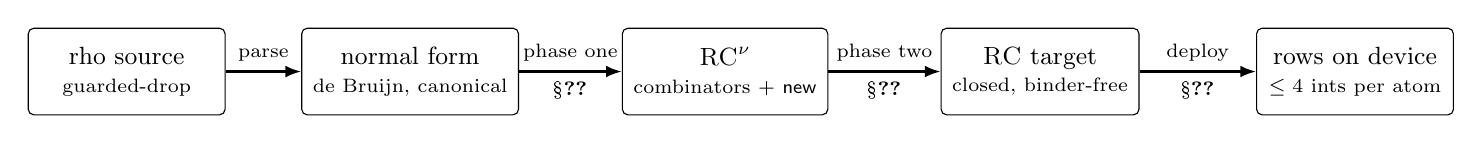
\begin{tikzpicture}[
  box/.style={draw, rounded corners=2pt, align=center, font=\small,
              minimum height=11mm, minimum width=25mm, inner sep=4pt},
  ar/.style={-{Latex[length=2mm]}, thick},
  lab/.style={font=\scriptsize, align=center}]
\node[box] (src) at (0,0) {rho source\\[-1pt]\scriptsize guarded-drop};
\node[box] (nrm) at (3.6,0) {normal form\\[-1pt]\scriptsize de Bruijn, canonical};
\node[box] (rcn) at (7.6,0) {$\rcnu$\\[-1pt]\scriptsize combinators $+\ \mathsf{new}$};
\node[box] (rc)  at (11.6,0) {$\rc$ target\\[-1pt]\scriptsize closed, binder-free};
\node[box] (mch) at (15.6,0) {rows on device\\[-1pt]\scriptsize $\le 4$ ints per atom};
\draw[ar] (src) -- node[above,lab]{parse} (nrm);
\draw[ar] (nrm) -- node[above,lab]{phase one} node[below,lab]{\S\ref{sec:phase1}} (rcn);
\draw[ar] (rcn) -- node[above,lab]{phase two} node[below,lab]{\S\ref{sec:phase2}} (rc);
\draw[ar] (rc) -- node[above,lab]{deploy} node[below,lab]{\S\ref{sec:machine}} (mch);
\end{tikzpicture}}
\caption{The compilation pipeline. Phase one removes the input binder by
reflection; phase two removes the name binder by run-time addressing; the
deployed state is a multiset of fixed-width rows over interned names.}
\label{fig:pipeline}
\end{figure}

\paragraph{What we do not claim.} We do not report wall-clock speedups over a
tuned sequential interpreter. Our GPU machine runs, and its step traces are
identical to those of the host machine, but our evaluation hardware is a
software Vulkan driver, and wall-clock numbers from it would be meaningless.
We instead measure the quantity on which any speedup from this route
depends: the width of compiled programs, meaning the number of rewrites per
bulk-synchronous step (\S\ref{sec:eval}). Whether real rho workloads are wide
is an empirical question our benchmarks do not settle, and we say so.

% ======================================================================
\section{The Rho Calculus}
\label{sec:rho}

The rho calculus~\cite{MeredithRadestock05} is an asynchronous name-passing
calculus in which names are not atoms but quoted processes. Its name is an
acronym, for the \emph{reflective higher-order} calculus, and a pun on the
letter after $\pi$.

\begin{definition}[Syntax]
\[
  P,Q \;::=\; \nil \;\mid\; \inp{y}{x}{P} \;\mid\; \out{x}{P}
        \;\mid\; \drp{x} \;\mid\; P \mid Q
  \qquad\qquad
  x,y \;::=\; \quo{P}
\]
\end{definition}

An output $\out{x}{P}$ sends a process, and the receiver binds its
quotation: in $\inp{y}{x}{Q}$ the variable $y$ ranges over names, and
$\drp{y}$ runs the process that $y$ quotes. Structural congruence $\scong$
makes $(\mid,\nil)$ a commutative monoid up to $\alpha$-equivalence. Name
equivalence $\nameq$ is the least congruence on names with
$\quo{\drp{x}} \nameq x$ and $\quo{P} \nameq \quo{Q}$ whenever $P \scong Q$.
Substitution decodes at the drop:
$(\drp{y})\{\quo{Q}/y\} = Q$, with the structural clauses otherwise.
Reduction is the single rule
\[
  \frac{x_{t} \nameq x_{s}}
       {\inp{y}{x_{t}}{P} \mid \out{x_{s}}{Q} \;\red\; P\{\quo{Q}/y\}}
\]
closed under parallel composition and $\scong$. We assume source programs are
\emph{guarded-drop}: every $\drp{x}$ has $x$ bound by an enclosing input, a
property preserved by reduction.

The calculus has no name restriction. Fresh names are obtained by quotation:
the name $\quo{P}$ is fresh for any process in which it does not occur, and
code can manufacture such names at run time. It is Turing complete; the
recursion combinator $D_{x} = \inp{y}{x}{(\out{x}{\drp{y}} \mid \drp{y})}$
behaves as a replication server when sent itself as a message, since each
reception re-sends its own quotation and runs it.

\paragraph{What makes it hard to run in parallel.}
Four things, which correspond to the four properties listed in
\S\ref{sec:intro}. A process is a tree of arbitrary shape, so the state of an
interpreter is a heap. A redex is found by matching an input against an
output whose channels are equal modulo $\nameq$, which is a recursive
comparison of trees modulo commutativity. Firing it substitutes under the
continuation's binders. And two inputs on one channel compete for one output,
so firing is a conflict-resolution problem. Tuple-space implementations of
the calculus solve each of these sequentially, with locks around the store.
The rest of the paper removes each of them by compilation.

% ======================================================================
\section{The Target: Name-Free Rho Combinators}
\label{sec:target}

The target calculus \rc{} has two sorts, names $\mathsf{N}$ and processes
$\mathsf{P}$, and is presented as an operational theory: formation rules,
equations, and named rewrite rules.

\subsection{Atoms and rules}

Processes are finite parallel compositions of \emph{atoms}. The base atoms are
\[
  \mm(a,v),\ \dd(a,b,c),\ \kk(a),\ \fw(a,b),\ \bl(a,b),\ \br(a,b),\
  \sy(a,b,c),\ \ev(a),\ \qq(a,p)
\]
with all arguments names except the payload $p$ of $\qq$. An atom $\mm(a,v)$
is a message carrying the name $v$ on the channel $a$. The six \emph{routers}
$\dd,\kk,\fw,\bl,\br,\sy$ consume a message and redirect, duplicate or
discard it. The \emph{destructor} $\ev$ consumes a message and runs the
process its payload quotes. The \emph{store} $\qq(a,p)$ holds a process that
only a forwarder can release. The equations are those of a commutative monoid
on $\mid$, together with $\quo{\drp{a}} = a$ and $\drp{\quo{p}} = p$; the
last makes quote and drop inverse, so a message payload may be a name, and
every argument of every atom other than a store is a name. The rules are
in Figure~\ref{fig:rules}.

\begin{figure}[t]
\small
\[
\begin{array}{@{}l@{\qquad}l@{}}
 \mathsf{dist}:\ \dd(a,b,c) \mid \mm(a,v) \red \mm(b,v) \mid \mm(c,v)
   & \mathsf{bind_l}:\ \bl(a,b) \mid \mm(a,v) \red \fw(v,b)\\
 \mathsf{kill}:\ \kk(a) \mid \mm(a,v) \red \nil
   & \mathsf{bind_r}:\ \br(a,b) \mid \mm(a,v) \red \fw(b,v)\\
 \mathsf{forward}:\ \fw(a,b) \mid \mm(a,v) \red \mm(b,v)
   & \mathsf{synch}:\ \sy(a,b,c) \mid \mm(a,v) \red \fw(b,c)\\
 \mathsf{eval}:\ \ev(a) \mid \mm(a,v) \red \drp{v}
   & \mathsf{quote}:\ \fw(a,b) \mid \qq(a,p) \red \mm(b,\quo{p})\\[3pt]
 \multicolumn{2}{@{}l@{}}{\mathsf{make}_{\mid}:\ \cons_{\mid}(a,b,c) \mid
   \mm(a,\quo{p}) \mid \mm(b,\quo{r}) \red \mm(c,\quo{(p \mid r)})}\\
 \multicolumn{2}{@{}l@{}}{\mathsf{make}_{A}:\ \cons_{A}(a_{1},\dots,a_{n},f)
   \mid \mm(a_{1},v_{1}) \mid \cdots \mid \mm(a_{n},v_{n})
   \red \mm(f,\quo{A(v_{1},\dots,v_{n})})
   \quad \text{each base shape } A}\\
 \multicolumn{2}{@{}l@{}}{\mathsf{inst}:\ \inst(a,f,C) \mid \mm(a,v) \red
   \mm(f,\quo{C[v]})
   \quad C \text{ a context, holes at names}}
\end{array}
\]
\caption{The rules of \rc{}, closed under $\mid$ and the equations, with
subjects matched up to $\nameq$. The six router rules and
$\mathsf{quote}$ (class~(a)) permute existing names; $\mathsf{make}$ and
$\mathsf{inst}$ (class~(b)) build a name; $\mathsf{eval}$ (class~(c)) opens
one.}
\label{fig:rules}
\end{figure}

\subsection{Three repairs to the published calculus}

The combinators descend from an unpublished draft~\cite{AnonOriginal} that
proposed them as a binder-free target for the rho calculus. Three changes
are needed before they can serve as one, and each matters to the machine.

\paragraph{The drop is not the guard.} The draft wrote the destructor and the
drop with one symbol, and kept $\drp{\quo{p}} = p$. Since every name is
$\quo{Q}$ for some $Q$, the destructor at $\quo{Q}$ is then equal to $Q$
itself, so for all $P,Q$
\[
  Q \mid \mm(\quo{Q},\quo{P}) \;\red\; P ,
\]
and any running process can be annihilated by anyone who knows its
quotation. Keeping $\ev$ and $\drp{-}$ as distinct constructors repairs this
and leaves the equation available. We use it: with $\drp{\quo{p}} = p$ a
payload is a name, hence an integer on the machine, and every atom is a
fixed-width row.

\paragraph{Names must be built as well as opened.} Without the constructors,
no rule produces a name that was not already present in the redex,
hereditarily. Rho reduction does so constantly: substituting into
$\quo{(\drp{y} \mid R)}$ yields $\quo{(Q \mid R)}$, a name in neither
participant. So no constructor-free combinator term is equivalent to, for
instance, $\inp{y}{a}{\out{\quo{(\drp{y} \mid \drp{y})}}{\nil}}$, and the
draft's calculus cannot encode the rho calculus at all. The family
$\cons_{A}$, one member per atom shape, restores the missing capability;
$\cons_{A}$ assembles the quotation of an $A$-node from the quotations of its
children (\S\ref{sec:lattice}).

\paragraph{Instantiation of a context.} The combinator $\inst$ builds, from
one received name $v$, the quotation of a whole context $C$ with $v$ in every
hole. It is derivable from the constructor family by chaining, so it adds no
expressive power to the calculus as a term algebra. It is nevertheless
primitive in our target, for a reason that only appears on a parallel
machine and that \S\ref{sec:phase2} makes precise.

\subsection{Rule classes}
\label{sec:classes}

The rules fall into three classes by what they ask of the machine.
\emph{Class (a)}: $\mathsf{dist}$, $\mathsf{kill}$, $\mathsf{forward}$,
$\mathsf{bind_l}$, $\mathsf{bind_r}$, $\mathsf{synch}$ and $\mathsf{quote}$
produce a fixed multiset of atoms over names in the premise; on the machine
they are field copies. \emph{Class (b)}: the constructors and $\inst$ produce
one message whose payload is a \emph{new} name, obtained by hash-consing a
term built from premise names. \emph{Class (c)}: $\mathsf{eval}$ is the only
rule whose conclusion has a size that depends on the value of a name; on the
machine it is a table read. The distinction recurs in \S\ref{sec:lattice},
where it separates what can be precomputed from what must be generated
lazily.

% ======================================================================
\section{Compilation}
\label{sec:compile}

The translation removes two binders in turn. Phase one compiles into
$\rcnu$, the combinators extended with a name binder
$(\mathsf{new}\,z)P$, much as \citet{Yoshida02} compiles the $\pi$-calculus
into combinators that keep $\mathsf{new}$. Phase two removes $\mathsf{new}$.
The split is not a convenience: \S\ref{sec:positional} shows that a
single-phase translation which invents apparatus names by syntactic position
is unsound.

\subsection{Phase one: eliminating the input binder by reflection}
\label{sec:phase1}

An input $\inp{y}{x}{P}$ must wait for a message on $x$, then run $P$ with the
received name in place of $y$. The combinators have no binder, so both halves
need a construction: something that holds $P$ until the message arrives, and
something that delivers the received name to each place in $P$ that uses it.

\begin{definition}[Gate and distributor]
For fresh $b,c$ put $G(p,S) := (\mathsf{new}\,b,c)\,(\sy(p,b,c) \mid \qq(b,S)
\mid \ev(c))$. A \emph{distributor} $D(x;p_{0},\dots,p_{k})$ is any binary tree
of $k$ atoms $\dd$, with fresh internal channels, whose root consumes at $x$
and whose leaves are $p_{0},\dots,p_{k}$.
\end{definition}

\begin{lemma}[Gate]
\label{lem:gate}
$G(p,S)$ has no reduction and is not a message. For any $v$,
\[
  G(p,S) \mid \mm(p,v)
  \;\red\; \fw(b,c) \mid \qq(b,S) \mid \ev(c)
  \;\red\; \mm(c,\quo{S}) \mid \ev(c)
  \;\red\; S ,
\]
and these are the only reductions available. $D(x;\vec p) \mid \mm(x,v)$
reduces in $k$ steps to $\mm(p_{0},v) \mid \cdots \mid \mm(p_{k},v)$, and in
$h$ bulk-synchronous steps, where $h$ is the height of the tree.
\end{lemma}

The gate stores the continuation as a quoted process inside $\qq$, which only
a forwarder can read, and $\sy$ produces that forwarder when the trigger
arrives. The continuation is never rewritten, only stored and released.
\citet[rules (I), (V), (VI)]{Yoshida02}, lacking reflection, must instead
delay each atom of the continuation behind its own synchroniser and split at
every parallel composition.

The distributor supplies copies of the received name. Occurrences of the
bound name $y$ in the body fall into five kinds (Table~\ref{tab:links}). For
the $i$-th occurrence the translation allocates a proxy $c_{i}$, rewrites the
occurrence inside the stored body, and emits a \emph{link} outside the gate
that connects the distributor's $i$-th leaf to the proxy.

\begin{table}[t]
\small
\begin{tabular}{@{}llll@{}}
\toprule
 & occurrence of $y$ in the body & rewritten in the stored body & link\\
\midrule
(o1) & input subject, $\inp{z}{y}{S}$ & subject becomes $c_{i}$ & $\bl(p_{i},c_{i})$\\
(o2) & output subject, $\out{y}{S}$ & subject becomes $c_{i}$ & $\br(p_{i},c_{i})$\\
(o3) & forwarded name, $\out{v}{\drp{y}}$ & atom deleted & $\fw(p_{i},\enc{v})$\\
(o4) & drop, $\drp{y}$ & becomes $\ev(c_{i})$ & $\fw(p_{i},c_{i})$\\
(o5) & inside $\quo{S}$, $y \in \fn(S)$ & subject becomes $c_{i}$
     & chain rebuilding $\quo{\enc{S}}$\\
\bottomrule
\end{tabular}
\caption{Occurrence kinds and their links. When several kinds meet in one atom,
the atom is deleted and the links are emitted together.}
\label{tab:links}
\end{table}

\begin{definition}[Phase one]
\label{def:phase1}
On names, $\enc{\quo{P}} := \quo{\enc{P}}$. On processes,
$\enc{\nil} = \nil$, $\enc{P \mid Q} = \enc{P} \mid \enc{Q}$,
$\enc{\out{x}{P}} = \mm(\enc{x},\quo{\enc{P}})$, and
\[
  \enc{\inp{y}{x}{P}} \;=\;
  (\mathsf{new}\,\vec p,\vec c,\vec q)\,
  \big(D(\enc{x};p_{0},\dots,p_{k}) \mid G(p_{0}, B) \mid L_{1} \mid \cdots
  \mid L_{k}\big)
\]
where $o_{1},\dots,o_{k}$ enumerate the free occurrences of $y$ in $P$, $L_{i}$
is the link of $o_{i}$, and $B$ is $\enc{P}$ with each occurrence rewritten as
in Table~\ref{tab:links}.
\end{definition}

Leaf $p_{0}$ triggers the gate; the others feed the links, which have
already fired, or are waiting at their proxies, by the time the body runs.
Kind (o4) is where the source's decoding substitution
$(\drp{y})\{\quo{Q}/y\} = Q$ and the target's $\mathsf{eval}$ rule meet:
the link forwards the received name to $c_{i}$, and the $\ev(c_{i})$ left in
the body opens it. Kind (o5) is the only one that constructs a name, and the
chain uses one constructor per node on the path from the occurrence to the
root of $S$.

\begin{proposition}[Size]
\label{prop:linear}
$|\enc{P}| = O(|P|)$, counting atoms. For
$P_{d} = \inp{x_{1}}{a}{\cdots \inp{x_{d}}{a}{\nil}}$,
$|\enc{P_{d}}| = 3d+1$, while Yoshida's elimination yields $(3^{d-1}+1)/2$
atoms.
\end{proposition}

\begin{proof}[Proof sketch]
An input contributes $k$ distributor atoms, three gate atoms and $k$ links,
where $k$ is the number of occurrences of its bound name, and its body is
translated once and stored once. Summing $k$ over binders counts each
occurrence once, and an (o5) chain is linear in the quoted subterm. For
$P_{d}$, no prefix has an occurrence. Yoshida's count satisfies $T(1)=1$,
$T(j+1) = 3T(j) - 1$: rule (I) inserts $n-1$ duplicators for a body of $n$
atoms and rule (VI) doubles each atom.
\end{proof}

The distributor can be any binary tree of $\dd$ atoms, and the original
formulation used a left comb, whose height is $k$. Since every copy of the
received name must pass through the tree before the corresponding occurrence
can act, the height is on the critical path of every instance. A balanced
tree has height $\lceil \log_{2}(k+1) \rceil$ with the same number of atoms.
The choice is invisible to the correctness argument, which uses only
Lemma~\ref{lem:gate}'s conclusion, and it matters a great deal on a
bulk-synchronous machine (\S\ref{sec:eval-dist}).

\subsection{Why positional apparatus is unsound}
\label{sec:positional}

Phase one's output still binds names. A tempting shortcut is to replace each
bound name by a name computed from its syntactic position, which is fresh for
the program because it quotes the position. The following program shows why
that fails. Let $R = \inp{y}{a}{\out{y}{\drp{y}}}$, which sends on the received
channel the process that channel quotes, and let
\[
  W \;=\; \inp{z}{b}{(\drp{z} \mid \drp{z})} \mid \out{b}{R}
      \mid \out{a}{X} \mid \out{a}{Y} .
\]
The communication on $b$ runs two copies of $R$, which in the source are
$\alpha$-distinct. One takes $\quo{X}$, the other $\quo{Y}$, and
$W \wred \out{\quo{X}}{X} \mid \out{\quo{Y}}{Y}$.

$R$'s single occurrence of $y$ is both an output subject and a forwarded
name, kinds (o2) and (o3), so its two links share one proxy $c$. Under
positional naming, both copies of $R$ are instantiated from the same quoted
text and carry the same $c$. After the links fire, the soup contains
\[
  \fw(c,\enc{\quo{X}}) \mid \fw(c,\enc{\quo{Y}}) \mid
  \mm(c,\enc{\quo{X}}) \mid \mm(c,\enc{\quo{Y}})
\]
and nothing pairs a forwarder with the message from its own copy. A run can
produce $\out{\quo{X}}{Y} \mid \out{\quo{Y}}{X}$, which an observer listening
on $\quo{X}$ distinguishes from the source. On our implementation the
positional scheme produces this crossed result on 49 of 100 random schedules
of $W$ (\S\ref{sec:eval-correct}). The underlying invariant is the
distinction between \emph{occurrences}, which positional naming separates,
and run-time \emph{instances}, which it does not. A binder separates both,
because two instances of $(\mathsf{new}\,c)P$ are $\alpha$-distinct. Phase one
keeps the binder for that reason, and phase two must eliminate it without
giving the property back.

\subsection{Phase two: eliminating the name binder by run-time addressing}
\label{sec:phase2}

Phase two runs every instance of compiled code at an \emph{address}, a name it
receives at run time, and derives its private names from that address. We
call a \emph{unit} any piece of phase-one output whose own level binds names:
the top level, the body stored in a gate, and any quoted process that
contains an input.

\paragraph{Addresses.} Fix two static constant names and write $\sigma\cdot w$
for the name obtained from $\sigma$ by the path $w \in \{0,1\}^{*}$, where
each bit applies one of two injective name constructors with disjoint images,
$L\sigma = \quo{\mm(\sigma,\quo{\nil})}$ and $R\sigma = \quo{\mm(\sigma,K)}$
for a fixed $K \neq \quo{\nil}$. Distinct paths give distinct names, and if
neither of $\sigma,\tau$ is a prefix of the other their subtrees are
disjoint. The $j$-th bound name of a unit is assigned the leaf at path
$\gamma(j)$, the Elias gamma code of $j$~\cite{Elias75}. Gamma codes are
prefix-free, so the leaves of one unit are pairwise incomparable and every
spare address a unit hands to a child owns a subtree disjoint from its
siblings'.

\paragraph{Erection.} Let $C_{U}$ be the context obtained from unit $U$'s
phase-one image by replacing each bound name $z_{j}$ with $\hole\cdot\gamma(j)$,
a path beneath the hole. The phase-two image of $U$ is
\[
  \enc{U}^{\sharp} \;:=\; A_{U} \;\mid\; \inst(r^{*},f^{*},C_{U}) \;\mid\; \ev(f^{*})
\]
where $A_{U}$ collects the atoms of $U$ that mention none of its bound names,
and $r^{*}, f^{*}$ are static channels. An address $\sigma$ arriving at
$r^{*}$ fires $\inst$, which delivers $\quo{C_{U}[\sigma]}$ at $f^{*}$, and
$\ev(f^{*})$ opens it. The instance is erected in two steps, whatever its
size, and all its private names are leaves beneath $\sigma$.

\paragraph{Supplying addresses.} An address must be available whenever code
with its own inputs is about to run, which happens at exactly two kinds of
site: a gate releasing a body that contains an input, and a drop $\drp{y}$,
which may run code received as a message. Phase one emits, for every such
site, a fresh $a$ with $\mm(r^{*},a)$ alongside the site; after phase two, $a$
is itself a leaf of the enclosing instance's address, so each run-time
instantiation receives an address posted by the event that caused it. Root
addresses for deployment are chosen larger than every name in the image and
pairwise prefix-incomparable.

\begin{lemma}[Freshness]
\label{lem:fresh}
If the root address exceeds every $\nameq$-normal name of the image, then no
allocated leaf occurs in the image, and no name constructed at run time by
an (o5) chain is a leaf.
\end{lemma}

\begin{proof}[Proof sketch]
Leaf construction strictly increases size on normal forms, which gives the
first claim. An (o5) chain builds only from names received on source
channels, and addresses never enter the payload of a source message, so no
constructed name mentions an address. The second clause is an obligation on
the compiler, and \tool{} checks it after compilation.
\end{proof}

\paragraph{Nested units need indexed holes.} A unit nested in another sits
inside its parent's context. If both use one hole marker, filling the parent
with its address also fills the child's hole, and every instance of the
child inherits the parent's names. This happens whenever an inner input
mentions an outer bound name, as in
$\inp{y}{a}{\inp{z}{b}{\out{y}{\drp{z}}}}$. Holes therefore carry a de Bruijn
index over enclosing contexts~\cite{deBruijn72}: $\hole_{0}$ is the innermost
context's hole, and $\inst$ fills its own hole while shifting deeper ones.

\subsection{Concurrent erection, and why fixed-arity constructors fail}
\label{sec:mixing}

Why is $\inst$ primitive, when the constructor family can build the same
names? Because on a machine that fires many redexes at once, how a name is
built matters as much as which name is built.

The natural erection without $\inst$ uses the family directly: to erect an
atom $A(z_{1},\dots,z_{m})$ of a unit at allocated leaves $t_{1},\dots,t_{m}$,
emit $\cons_{A}(t_{1},\dots,t_{m},f_{A}) \mid \ev(f_{A})$ and let an
allocation gadget deliver each leaf as a message on a statically named
channel. Every instance of the unit shares those static channels. With two
instances live at $\sigma$ and $\tau$, the constructor for the distributor atom
$\dd(a,p_{0},q_{1})$ can take $p_{0}$ from $\sigma$ and $q_{1}$ from $\tau$ and
erect $\dd(a,\sigma\cdot00,\tau\cdot01)$. From that point on, values cross
between instances, and the failure of \S\ref{sec:positional} returns. We
measure how often in \S\ref{sec:eval-erection}: often, and more often under
maximal-progress scheduling than under sequential choice, because a
bulk-synchronous step fires every enabled constructor while both instances'
leaves are present.

The condition that prevents this can be stated locally.

\begin{definition}[Single-address discipline]
\label{def:dstar}
Fix an instance at address $\sigma$. A redex \emph{joins at a static channel}
if one of the channels it consumes is static and two of its premises
contribute occurrences of $\sigma$ to the atoms it produces. A compiled image
satisfies the discipline if no reachable redex joins at a static channel.
\end{definition}

\begin{proposition}[Address multiplicity]
\label{prop:multiplicity}
Under the discipline, and with the rules of Figure~\ref{fig:rules} other
than $\inst$, no reachable atom contains two occurrences of an address
$\sigma$. Hence no atom mentioning two leaves beneath $\sigma$ is ever erected
--- in particular, neither the distributor atom $\dd(q_{1},p_{1},q_{2})$ nor
the gate's $\sy(p_{0},b,c)$.
\end{proposition}

\begin{proof}
By induction on reduction. Initially the image is closed and the address
arrives as $\mm(r^{*},\sigma)$, one occurrence. Every rule other than $\inst$
builds its produced atoms from the consumer's arguments, the payloads of its
consumed messages, and static names; for $\mathsf{eval}$, the components of a
single payload. A produced atom with two occurrences of $\sigma$ must draw one
from each of two premises. At least one of those is a payload carrying
$\sigma$, consumed at a channel that, by the induction hypothesis applied to
the message atom, is free of $\sigma$ and hence static. The redex then joins at
a static channel, which the discipline excludes. A leaf beneath $\sigma$
contains exactly one occurrence of $\sigma$.
\end{proof}

A fixed-arity constructor places each input once. Building an atom that
mentions $\sigma$ twice from one copy of $\sigma$ requires duplicating it and
joining the copies again, and the join is the forbidden one. So the
difficulty lies not in the arity of the atoms but in the premise count of the
rule: a two-premise rule can pair premises from different instances, since
matching is on subject names alone, while a one-premise rule cannot mispair
anything. $\inst$ has one premise and places its input at every hole, so its
image satisfies the discipline by construction, and addresses at $r^{*}$ are
then interchangeable.

\begin{lemma}[Permutation]
\label{lem:perm}
Let instances run at pairwise prefix-incomparable addresses in an image
erected by $\inst$. Every reachable configuration is one in which each
instance's atoms mention leaves of a single address, and reachable
configurations differ from the uncrossed ones by a permutation of addresses
among instances.
\end{lemma}

We note one alternative. A \emph{curried} constructor
$\cons^{*}_{A}[\vec w](t,f) \mid \mm(t,\sigma) \red
\mm(f,\quo{A(\sigma\cdot w_{1},\dots,\sigma\cdot w_{n})})$ also has one
premise and keeps the signature fixed-arity. It erects one atom per rule, so a
unit costs a fan-out tree of copies of $\sigma$ plus one constructor per atom,
and it cannot erect a stored body with two atoms that mention the unit's names
without a join at a derived channel. We implement it as an option and compare
the two in \S\ref{sec:eval-erection}; the device targets $\inst$ only.

\subsection{Correctness}
\label{sec:correct}

We state correctness as full abstraction for an observational equivalence
defined by context-labelled transitions~\cite{Sewell98,LeiferMilner00}. For a
calculus with contexts $\Ctx$ and a class of observers
$\mathcal{D} \subseteq \Ctx$, write $P \xrightarrow{C} P'$ when $C[P] \red P'$,
and let $\bisim_{\mathcal{D}}$ be the largest symmetric relation such that
$P \bisim_{\mathcal{D}} Q$ and $P \xrightarrow{C} P'$ with $C \in \mathcal{D}$
imply $C[Q] \wred Q'$ with $P' \bisim_{\mathcal{D}} Q'$. On the source the
observers are all rho contexts; on the target, the images $\enc{\Ctx}$ of rho
contexts.

\begin{theorem}[Full abstraction relative to encoded contexts]
\label{thm:fullabs}
For all guarded-drop rho processes $P,Q$,
\[
  P \bisim_{\Ctx} Q
  \quad\Longleftrightarrow\quad
  \enc{P}^{\sharp} \bisim_{\enc{\Ctx}} \enc{Q}^{\sharp}.
\]
\end{theorem}

\begin{proof}[Proof sketch]
The argument follows \citet{AnonRhocomb}. The translation is compositional on
the nose, $\enc{C[P]} = \enc{C}[\enc{P}]$. An erected input is inert and
contains no message. Within one instance every allocated name is the subject of
at most one atom and carries at most one message, so each link is a one-shot
forwarder, and a term with finitely many links added is bisimilar to one with
the links discharged (\emph{link expansion}). The key lemma is \emph{release}:
an erected input, given a message on its channel, reduces in a number of
steps linear in $k$ to a term that is a link expansion of the translation of
the substituted body, and no other reduction sequence is available up to the
order of independent steps. Kinds (o1)--(o3) contribute forwarders, (o4)
contributes exactly the decoding substitution, and (o5) rebuilds the
substituted quotation node by node. \emph{Address independence} ---
instances at incomparable addresses are bisimilar under the bijection
$\sigma\cdot w \mapsto \tau\cdot w$, because an encoded context never names an
allocated leaf --- together with Lemma~\ref{lem:perm} absorbs the permutation
of addresses at $r^{*}$. The forward direction builds a bisimulation from
release and link expansion; the backward direction reads release left to
right, so a distinguishing source context yields a distinguishing encoded
context.
\end{proof}

\begin{proposition}[The relativisation is forced]
\label{prop:forced}
There are $P \bisim_{\Ctx} Q$ and a combinator context $C \notin \enc{\Ctx}$
with $C[\enc{P}^{\sharp}] \not\bisim C[\enc{Q}^{\sharp}]$.
\end{proposition}

\begin{proof}
An arbitrary combinator context can name the gate channel $b$ of a translated
input and install $\fw(b,u)$, extracting the stored continuation at an
observable $u$ (Lemma~\ref{lem:gate}). Two source terms differing only in a
continuation that is never reached are then distinguished. No encoded context
installs such a forwarder.
\end{proof}

The same shape of result holds for the fully abstract encoding of the
$\pi$-calculus in the rho calculus~\cite{AnonNowns,Lybech22}, for the same
reason: the target manufactures names the source lacks, and an unrestricted
observer can use them. It is also where the store $\qq$ earns its place. With
the continuation held as a message $\mm(b,\quo{B})$ rather than a store, no
action by the observer would be needed; the store is the continuation made
quiet.

% ======================================================================
\section{A Bulk-Synchronous Machine for the Combinators}
\label{sec:machine}

\subsection{States are multisets of rows}
\label{sec:states}

A \emph{species} is a head symbol applied to a tuple of names, modulo
$\nameq$. A target state is a finite multiset of species: the multiset of
top-level atoms of the state's drop-free normal form is a complete invariant
for structural congruence~\cite{AnonLogic}, so $P \scong Q$ iff their
multisets agree. The monoid laws of $\mid$ are therefore the algebra of the
data structure, and $\drp{\quo{p}} = p$ and $\quo{\drp{a}} = a$ are discharged
once, when names are interned. Matching modulo structural congruence, a
recurring cost for a direct interpreter, costs nothing here.

Names are processes, and processes are multisets of species, so the index set
of the representation indexes itself:
$\mathcal{N} \cong M_{\mathrm{fin}}(\mathcal{S})$ with
$\mathcal{S} = \coprod_{A} \mathcal{N}^{\mathrm{ar}(A)}$. This is reflection
seen from the data structure, and it is why no finite matrix can be written
down in advance. The machine realises $\mathcal{N}$ by an \emph{intern
table}, a bijection between integers and canonical component multisets with
two directions: $\mathsf{quote}$, hash-consing~\cite{FilliatreConchon06}, used
by class (b) rules; and $\mathsf{drop}$, a table read, used by class (c).
Interning is structural: a name is stored as a row whose components are the
indices of its children, so building a leaf one level beneath an address of
any depth is one new entry, and no hash of a full encoding is computed on the
hot path. Which integer a name receives depends on the order of insertion; it
is a gauge freedom, and the machine never lets an integer comparison stand in
for a semantic distinction between runs.

With names interned, every atom is a head symbol and at most four integer
arguments: three for most shapes, four for $\cons_{\dd}$ and $\cons_{\sy}$,
and for $\inst$ its two channels and the index of its interned context. A state is a structure of arrays, one table per shape, one column per
argument slot.

\subsection{The rules as an operator}
\label{sec:lattice}

Viewing a state as a basis vector $|\gamma\rangle$ of the free module on
multisets, each rule $r$ with premise multiset $L_{r}$ and conclusion $R_{r}$
defines an operator
$H_{r} = \sum_{\theta} \big(\prod_{\beta \in R_{r}\theta} a^{\dagger}_{\beta}\big)
\big(\prod_{\alpha \in L_{r}\theta} a_{\alpha}\big)$, with $a^{\dagger}$ and $a$
adding and removing one occurrence of a species~\cite{Doi76,BaezBiamonte18}.
The transfer operator $T = \sum_{r} H_{r}$ represents the rules alone,
independently of any term, and the reduction graph of $\gamma$ is the orbit of
$|\gamma\rangle$ under $T$. Its matrix elements count derivations by the
mass-action law: the combinators are a chemical reaction network whose
reactions are generated from the shape table.

$T$ is never materialised. It is useful because the invariants that separate
subsets of the combinators by expressive power are exactly the finiteness
conditions of $T$.

\begin{theorem}[The expressiveness lattice classifies the operator]
\label{thm:three}
Let $\gamma$ be a state over a set of atoms.
\begin{enumerate}[label=(\roman*),leftmargin=2.2em]
\item \emph{Index set.} Every name in a reduct of $\gamma$ lies in the closure
  of the names of $\gamma$ under the node shapes of the constructors present.
  Without constructors the reachable species are finite; with them they are
  the free algebra on the initial names, generated on demand.
\item \emph{Nilpotency.} Weight $\bl,\br,\sy$ at 2 and every other non-message
  atom at 1. Every rule except $\mathsf{eval}$ strictly decreases the weight.
  Without $\ev$ the reachable operator is strictly block upper triangular,
  $T^{\Wt(\gamma)+1} = 0$, and reachability is the terminating Neumann series
  $(\mathbf{1}-T)^{-1} = \prod_{i} (\mathbf{1} + T^{2^{i}})$, computable by
  $\lceil \log_{2}(\Wt(\gamma)+1)\rceil$ sparse squarings.
\item \emph{Occupation.} Without $\dd$ and $\ev$, the combined number of
  messages and stores does not increase.
\end{enumerate}
\end{theorem}

Each clause is the lemma that proves an edge of the expressiveness lattice,
read as a statement about $T$: (i) is the name-closure lemma, which makes the
constructor edges strict, and (ii) is the proof that without $\ev$ the
calculus is strongly normalising, hence not Turing complete. The destructor
$\ev$ therefore has three characterisations: it carries Turing power, it is
the unique rule that breaks the grading, and it is the unique rule whose
operator cannot be written schematically, since its image depends on the
contents of the intern table. Every compiled input contains $\ev$ in its gate,
so clause (ii) applies to input-free programs and hand-written terms only;
compiled programs are run from the frontier, which is what the machine below
does.

\subsection{Redex finding is a join}
\label{sec:joins}

For each shape $A$ and slot $j$ let $M^{A}_{j}$ be the Boolean matrix with
$M^{A}_{j}[i,n] = 1$ iff the $i$-th occurrence of $A$ carries name $n$ in slot
$j$. The whole family has one nonzero per argument, so it is the size of the
term. Every rule is a conjunction of atom premises that share names, so redex
finding is a relational join on these matrices. The seven two-premise rules
against a message are the product $M^{C}_{0} (M^{\mm}_{0})^{\top}$; the
$\mathsf{quote}$ rule is $M^{\fw}_{0} (M^{\qq}_{0})^{\top}$; an $n$-ary
constructor is $n$ such products followed by a row-wise product with a mask
enforcing distinct message occurrences. Two redexes \emph{conflict} if they
consume a common occurrence, so with $B$ the redex--occurrence incidence
matrix the conflict graph is the off-diagonal pattern of $BB^{\top}$. The whole
per-step analysis is two rounds of sparse joins on term-sized operands. No
matrix whose dimension is the number of states appears.

\subsection{The parallel step}
\label{sec:step}

\begin{definition}[Step]
Redexes enabled in $\gamma$ are \emph{independent} if the occurrences they
consume are disjoint. A \emph{step} $\gamma \Rightarrow_{S} \gamma'$ fires a set
$S$ of pairwise independent redexes, removing every consumed occurrence and
adding every produced atom.
\end{definition}

\begin{lemma}[Diamond]
\label{lem:diamond}
If $r_{1},r_{2}$ are independent and enabled in $\gamma$, each remains enabled
after the other fires, and both orders yield the same state up to the
canonical bijection on interned names.
\end{lemma}

\begin{proof}
Firing removes only consumed occurrences, so disjointness preserves each
premise. The produced atoms of $r_{i}$ are a function of the occurrences it
consumes and of the intern table, whose contributions are independent of
insertion order up to the canonical bijection. Both orders give
$\gamma - L_{r_{1}} - L_{r_{2}} + R_{r_{1}} + R_{r_{2}}$.
\end{proof}

\begin{theorem}[Step soundness]
\label{thm:sound}
If $\gamma \Rightarrow_{S} \gamma'$ then $\gamma \wred \gamma'$ by a sequential
derivation firing exactly the members of $S$, in any order, and all such
orders agree. Consequently a run of $k$ steps performs $\sum_{i} |S_{i}|$
rewrites, the available speedup over a sequential interpreter is the mean
step width, and $k$ is bounded below by the causal depth of the derivation.
\end{theorem}

\begin{proof}
Induction on $|S|$ with Lemma~\ref{lem:diamond}.
\end{proof}

The converse fails deliberately. Firing a \emph{maximal} independent set
excludes interleavings in which an enabled, unconflicted redex waits, and when
redexes conflict, choosing which one enters $S$ is choosing a schedule. Maximal
progress is therefore a scheduler, not a semantics: the machine explores a
subset of the source's behaviours, each of which is a genuine behaviour by
Theorem~\ref{thm:sound}. For the rho calculus, whose nondeterminism is
precisely the resolution of races on channels, this is the expected contract,
and it is the contract a tuple-space implementation offers when its cores
race. We randomise priorities afresh at every step, as Luby's algorithm
does~\cite{Luby86}, so that no enabled redex is starved by a fixed order.

\begin{figure}[t]
\centering
\resizebox{\textwidth}{!}{%
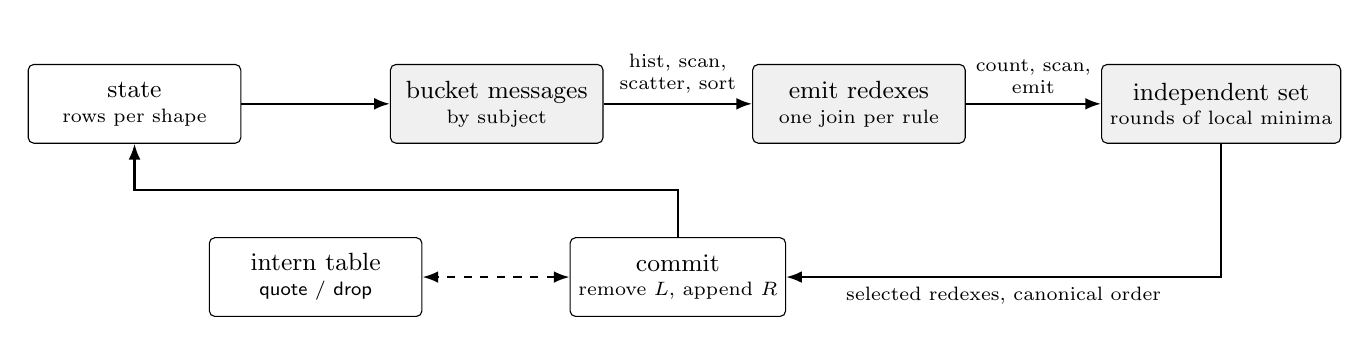
\begin{tikzpicture}[
  box/.style={draw, rounded corners=2pt, align=center, font=\small,
              minimum height=10mm, minimum width=27mm, inner sep=3pt},
  dev/.style={box, fill=black!6},
  ar/.style={-{Latex[length=2mm]}, thick},
  lab/.style={font=\scriptsize, align=center}]
\node[box] (st)  at (0,0)    {state\\[-2pt]\scriptsize rows per shape};
\node[dev] (bk)  at (4.6,0)  {bucket messages\\[-2pt]\scriptsize by subject};
\node[dev] (rd)  at (9.2,0)  {emit redexes\\[-2pt]\scriptsize one join per rule};
\node[dev] (mis) at (13.8,0) {independent set\\[-2pt]\scriptsize rounds of local minima};
\node[box] (cm)  at (6.9,-2.2) {commit\\[-2pt]\scriptsize remove $L$, append $R$};
\node[box] (it)  at (2.3,-2.2) {intern table\\[-2pt]\scriptsize $\mathsf{quote}$ / $\mathsf{drop}$};
\draw[ar] (st) -- node[below,lab,yshift=-7mm]{} (bk);
\node[lab] at (2.3,0.85) {};
\draw[ar] (bk) -- node[above,lab]{hist, scan,\\scatter, sort} (rd);
\draw[ar] (rd) -- node[above,lab]{count, scan,\\emit} (mis);
\draw[ar] (mis) |- node[pos=0.75,below,lab]{selected redexes, canonical order} (cm);
\draw[ar] (cm.north) -- ++(0,0.6) -| (st.south);
\draw[{Latex[length=2mm]}-{Latex[length=2mm]},dashed,thick] (cm) -- (it);
\end{tikzpicture}}
\caption{One machine step. Shaded stages run on the device as generated WGSL
kernels; every arrow between them is a bulk-synchronous barrier. The dashed
arrow is the only access to shared mutable state, used by class (b) and (c)
rules.}
\label{fig:step}
\end{figure}

% ======================================================================
\section{Implementation}
\label{sec:impl}

\tool{} is a Rust workspace of eight crates, about 7{,}800 lines excluding a
vendored parser. Its pipeline follows Figure~\ref{fig:pipeline}.

\paragraph{Front end.} A parser and normaliser for the kernel of the rho
calculus produce a canonical form with de Bruijn indices, so that
$\alpha$-equivalent programs have byte-identical encodings.

\paragraph{Phase one.} This phase is a homomorphism on the normal form into an IR for
$\rcnu$ with its own $\mathsf{New}$ node and a nameless encoding, so
$\alpha$-equivalence is equality of encodings. It classifies occurrences as in
Table~\ref{tab:links}, emits the (o5) constructor chains, and posts an address
request at every release site.

\paragraph{Phase two.} This phase compiles each unit to its $\inst$ erection, with bound
names written as Elias-gamma leaves beneath de Bruijn-indexed holes. Four
post-passes fail compilation if violated: the single-address discipline; no
address feeding an (o5) chain (Lemma~\ref{lem:fresh}); no static channel
occurring as a value; and no hole outside a context. Two further schemes are
available for comparison: \emph{curried}, and \emph{positional}, which is the
unsound scheme of \S\ref{sec:positional} kept as a negative control.

\paragraph{Rule table.} The twenty rules are \emph{generated} from a table of
twenty-one shapes: nine base atoms, $\cons_{\mid}$, one constructor per base
shape, $\inst$, and the curried constructor. Each rule records its consumer
shape, its premises as (argument slot, message or store) pairs, and its
conclusion as a class (a) atom template, a class (b) encode template, or the
class (c) decode. The host machine, the GPU kernels and the manifest shipped
with each GPU bundle all read this one table.

\paragraph{Host machine.} States are structure-of-arrays tables per shape over
a structural intern table. Each step sorts redexes by a canonical key,
computes conclusions in that order, and interns any new names in a fixed
traversal order, so runs are deterministic given a seed and host and device
assign identical integers. Four resolvers are provided: maximal progress,
single redex by priority, single redex uniformly at random, and an
adversarial resolver that deliberately prefers redexes whose premises come
from different instances.

\paragraph{GPU machine.} The device backend uses wgpu (Vulkan, Metal or
DirectX~12) and WGSL kernels generated from the rule table, which enters the
shader as constant arrays: per rule, the consumer shape, the number of
premises, and for each premise the argument slot it joins on and whether it
reads a message or a store. A step dispatches twelve kernels
(Figure~\ref{fig:step}). Redex finding is a radix-partitioned hash join:
message and store rows are histogrammed by subject name, prefix-scanned,
scattered and sorted within buckets; each consumer row then counts its
candidate partners in the bucket of its joined slot, a second scan assigns
output offsets, and an emit kernel writes redex records of eight words each.
Selection is a greedy maximal independent set computed in rounds: each redex
draws a 64-bit priority from a SplitMix64 finaliser keyed by the seed, the
step number, its rule and the rows it consumes; each occurrence records the minimum priority among its
undecided redexes by three passes of 32-bit atomic minimum (high word, low
word, index); a redex that is the minimum at every occurrence it touches is
taken, and redexes touching a taken occurrence are excluded. Rounds repeat
until no redex is undecided, which yields exactly the set the sequential
greedy algorithm yields in priority order. The host then commits the step,
sharing the host machine's commit routine, so that the intern table stays on
the host. Device and host step traces are therefore identical by
construction of the selection and are checked to be so by test. Moving the
intern table behind a batched device-side insert-or-get is future work.

\paragraph{Artefacts.} Every stage can be saved and fed back in: a textual IR
after phase one, a canonical binary target after phase two whose header
records the scheme, the constructor subset the program uses and a marking
analysis, and a GPU bundle holding the deployed state, the generated kernels,
and a manifest with the rule table, buffer layout, dispatch sequence and a
reference trace summary that a device run must reproduce.

% ======================================================================
\section{Evaluation}
\label{sec:eval}

We ask four questions. \textbf{RQ1}: does the compiler preserve behaviour, and
do host and device agree? \textbf{RQ2}: do machine steps track causal depth
rather than work on compiled rho programs, and what does compilation cost in
rewrites? \textbf{RQ3}: what limits width, and can the compiler remove the limits it
creates? \textbf{RQ4}: how do the erection schemes compare under concurrent
instantiation?

\paragraph{Setup.} All runs use the release build of \tool{} under Rust
1.85 on Ubuntu 24.04, with the device backend on Mesa's software Vulkan
driver (llvmpipe, LLVM~20). Step counts, widths and redex counts are
properties of the machine semantics and are identical on any adapter; we do
not report times.

\subsection{RQ1: Correctness}
\label{sec:eval-correct}

The test suite comprises 48 tests in the workspace and 33 in the vendored
front end, all passing. The central checks are differential against a
reference reducer for the source calculus, comparing encoded observations at
quiescence.
\begin{itemize}[leftmargin=1.5em]
\item \emph{The regression term $W$} of \S\ref{sec:positional}, and a
  three-copy variant, agree with the source on all 100 seeds, and the crossed
  residue $\out{\quo{X}}{Y}$ never appears. Under the positional negative
  control, $W$ crosses on 49 of 100 seeds and the three-copy variant on 85.
\item \emph{A corpus of 19 programs} covering every occurrence kind, nested
  inputs, relays, (o5) chains, races, and received code with inputs run once
  and twice agrees with the source on 4 seeds on the host and 2 on the
  device, and gives identical observations at two different root addresses
  (address independence).
\item \emph{Adversarial scheduling.} Under the resolver that prefers
  cross-instance matches, $W$ and its variants show no disagreement in 100
  seeds each.
\item \emph{Host--device agreement.} Device and host step traces are
  identical on the regression terms and the corpus, and on every benchmark
  below the final state hashes agree.
\item \emph{Canonicity.} Programs differing by a permutation of parallel
  components compile to $\alpha$-equal phase-one images and byte-equal
  targets.
\end{itemize}

\subsection{RQ2: Width of compiled programs}
\label{sec:eval-width}

The width thesis of this approach is that the available speedup is the mean
number of rewrites per step, and nothing else. We therefore measure width on
five families of rho programs whose causal structure is known analytically,
each compiled by \tool{} and run to quiescence under maximal progress, with
three seeds (all measurements were seed-independent).
\begin{description}[leftmargin=1.5em,style=unboxed]
\item[fan$(n,d)$:] $n$ independent relay chains of depth $d$, each link
  $\inp{y}{c_{i,j}}{\out{c_{i,j+1}}{\drp{y}}}$. Causal depth $d$, width $n$.
\item[bcast$(h)$:] a broadcast tree of height $h$, each node
  $\inp{y}{c_{v}}{(\out{c_{2v}}{\drp{y}} \mid \out{c_{2v+1}}{\drp{y}})}$. Causal
  depth $h$, width $2^{h-1}$ at the last level.
\item[contend$(c)$:] $c$ inputs and $c$ outputs on one channel. Causal depth
  one, maximal contention.
\item[nested$(n,d)$:] $n$ clients each running $d$ nested inputs on a private
  channel. Causal depth $d$, width $n$.
\item[ship$(n)$:] higher-order. A process
  $\inp{z}{b}{(\drp{z} \mid \cdots \mid \drp{z})}$ with $n$ drops receives a
  piece of code containing an input, runs $n$ copies of it, and each copy
  serves one of $n$ client messages. This is $W$ at scale: every copy needs
  its own address and its own erection.
\end{description}

\begin{table}[t]
\small
\begin{tabular}{@{}lrrrrrr@{}}
\toprule
program & source comms & rewrites & parallel steps & max width & mean width & enum./fired\\
\midrule
fan$(1,8)$    &   8 &    42 & 20 &   3 &   2.1 & 1.00\\
fan$(4,8)$    &  32 &   162 & 20 &  12 &   8.1 & 1.00\\
fan$(16,8)$   & 128 &   642 & 20 &  48 &  32.1 & 1.00\\
fan$(64,8)$   & 512 & 2{,}562 & 20 & 192 & 128.1 & 1.00\\
\midrule
bcast$(2)$    &   3 &    23 &  9 &   6 &   2.6 & 1.00\\
bcast$(4)$    &  15 &   107 & 15 &  24 &   7.1 & 1.00\\
bcast$(6)$    &  63 &   443 & 21 &  96 &  21.1 & 1.00\\
bcast$(8)$    & 255 & 1{,}787 & 27 & 384 &  66.2 & 1.00\\
\midrule
nested$(1,4)$  &   4 &    20 & 20 &   1 &   1.0 & 1.30\\
nested$(4,4)$  &  16 &    74 & 20 &   4 &   3.7 & 2.30\\
nested$(16,4)$ &  64 &   290 & 20 &  16 &  14.5 & 6.30\\
nested$(64,4)$ & 256 & 1{,}154 & 20 &  64 &  57.7 & 22.3\\
\midrule
contend$(4)$  &   4 &    22 &  6 &   8 &   3.7 & 1.55\\
contend$(16)$ &  16 &    82 &  6 &  32 &  13.7 & 3.93\\
contend$(64)$ &  64 &   322 &  6 & 128 &  53.7 & 13.5\\
\midrule
ship$(1)$     &   2 &    15 & 13 &   2 &   1.2 & 1.00\\
ship$(4)$     &   5 &    45 & 14 &   6 &   3.2 & 1.53\\
ship$(16)$    &  17 &   165 & 26 &  11 &   6.3 & 2.59\\
ship$(64)$    &  65 &   645 & 74 &  11 &   8.7 & 7.36\\
ship$(256)$   & 257 & 2{,}565 & 266 & 11 &  9.6 & 26.6\\
\bottomrule
\end{tabular}
\caption{Width of compiled programs under maximal progress, with the
distributor of the original formulation (a left comb). \emph{Rewrites} is
the number of combinator rewrites, equal to the step count of a sequential
combinator interpreter; \emph{mean width} is rewrites per parallel step;
\emph{enum./fired} is redexes enumerated per redex fired.}
\label{tab:width}
\end{table}

Table~\ref{tab:width} gives the results. For fan, nested and contend, the
number of parallel steps is independent of the width parameter across a
64-fold range, and mean width grows linearly with it: the machine's depth is
the program's causal depth plus a constant for deployment and erection. For
bcast, parallel steps grow as $3h+3$ while rewrites grow as $2^{h}$; three
machine steps per level of the tree are the output message, the distributor
and the forward to the child's gate. Compilation multiplies the number of
rewrites by a constant: between 4.5 and 7 combinator rewrites per source
communication across the four first-order families. The machine gives this
back many times over as soon as width exceeds seven.

\subsection{RQ3: What limits width, and a fix}
\label{sec:eval-dist}

The ship family is the exception. Its parallel steps grow linearly with $n$,
and its mean width saturates below ten. The per-step trace locates the cause.
The receiving input $\inp{z}{b}{(\drp{z} \mid \cdots \mid \drp{z})}$ has $n$
occurrences of $z$, so its distributor has $n$ atoms, and in the original
formulation these form a chain: $\dd(x,p_{0},q_{1}) \mid \dd(q_{1},p_{1},q_{2})
\mid \cdots$. The chain releases one copy of the received code per step, so the
$n$ instances are erected one after another however wide the machine is. This
is a depth cost the compiler introduced, not one the program has: in the
source all $n$ drops fire in the same communication.

Replacing the chain with a balanced tree of the same $n$ atoms
(\S\ref{sec:phase1}) is a local change to phase one, and it leaves every
conclusion of Lemma~\ref{lem:gate} unchanged. With it, the full test suite
passes except the golden files, which record the old distributor's shape, and
host and device traces still agree. Table~\ref{tab:dist} and
Figure~\ref{fig:steps} show the effect. Parallel steps for ship$(256)$ fall
from 266 to 20, mean width rises from 9.6 to 128, and the number of rewrites is
unchanged. The other families are unaffected, since their inputs use each
bound name at most once or twice.

\begin{table}[t]
\small
\begin{tabular}{@{}lrrrrrr@{}}
\toprule
& \multicolumn{3}{c}{chain distributor} & \multicolumn{3}{c}{balanced distributor}\\
\cmidrule(lr){2-4}\cmidrule(lr){5-7}
program & steps & max width & mean width & steps & max width & mean width\\
\midrule
ship$(4)$   &  14 & 6  & 3.2 & 14 &   8 &   3.2\\
ship$(16)$  &  26 & 11 & 6.3 & 16 &  32 &  10.3\\
ship$(64)$  &  74 & 11 & 8.7 & 18 & 128 &  35.8\\
ship$(256)$ & 266 & 11 & 9.6 & 20 & 512 & 128.3\\
\bottomrule
\end{tabular}
\caption{The distributor's shape on the higher-order family. Rewrites are
identical in both columns (Table~\ref{tab:width}).}
\label{tab:dist}
\end{table}

\begin{figure}[t]
\centering
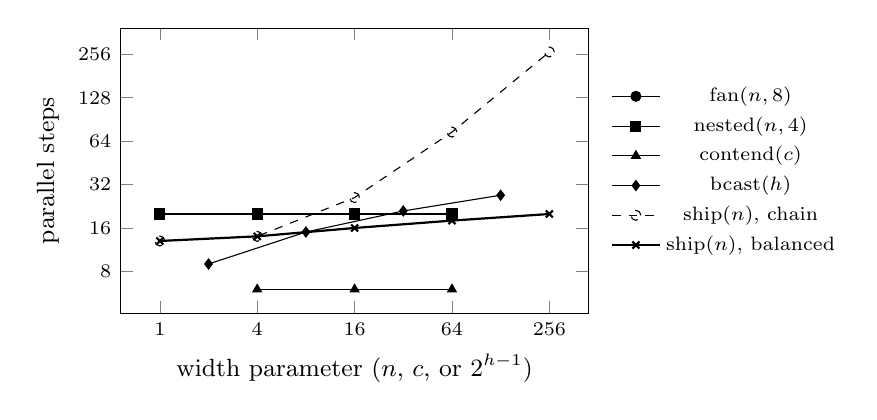
\begin{tikzpicture}
\begin{axis}[
  width=0.62\textwidth, height=5.2cm,
  xmode=log, log basis x=2, ymode=log, log basis y=2,
  xlabel={width parameter ($n$, $c$, or $2^{h-1}$)},
  ylabel={parallel steps},
  xtick={1,4,16,64,256}, xticklabels={1,4,16,64,256},
  ytick={4,8,16,32,64,128,256}, yticklabels={4,8,16,32,64,128,256},
  legend style={font=\scriptsize, at={(1.03,0.5)}, anchor=west, draw=none},
  tick label style={font=\scriptsize}, label style={font=\small},
  mark size=1.8pt]
\addplot[mark=*] coordinates {(1,20) (4,20) (16,20) (64,20)};
\addlegendentry{fan$(n,8)$}
\addplot[mark=square*] coordinates {(1,20) (4,20) (16,20) (64,20)};
\addlegendentry{nested$(n,4)$}
\addplot[mark=triangle*] coordinates {(4,6) (16,6) (64,6)};
\addlegendentry{contend$(c)$}
\addplot[mark=diamond*] coordinates {(2,9) (8,15) (32,21) (128,27)};
\addlegendentry{bcast$(h)$}
\addplot[mark=o, dashed] coordinates {(1,13) (4,14) (16,26) (64,74) (256,266)};
\addlegendentry{ship$(n)$, chain}
\addplot[mark=x, thick] coordinates {(1,13) (4,14) (16,16) (64,18) (256,20)};
\addlegendentry{ship$(n)$, balanced}
\end{axis}
\end{tikzpicture}
\caption{Parallel steps against width. Flat lines are the goal: depth
independent of the amount of parallel work. The chain distributor makes the
higher-order family linear; the balanced distributor makes it logarithmic.}
\label{fig:steps}
\end{figure}

\paragraph{Contention.} The last column of Table~\ref{tab:width} measures
work the machine does and discards. For contend$(c)$ the machine enumerates
$c^{2}$ candidate redexes on the shared channel and fires a perfect matching of
$c$ in one step, so the ratio grows linearly. The same effect appears for
nested and, after the distributor fix, for ship: $n$ instances request
addresses at the one static channel $r^{*}$, and the $n$ $\inst$ atoms and $n$
addresses there form $n^{2}$ candidate pairs (77 per fired redex for
ship$(256)$). Contention thus costs enumeration, not depth. For rules with a
single message premise the enumeration is avoidable in principle: within a
bucket, a matching between consumers and messages can be formed by pairing
ranks after one segmented scan, and for multi-premise rules worst-case-optimal
joins~\cite{Ngo18} apply. We have not implemented either, and until one is
implemented these families would be enumeration-bound on real hardware at
large $c$.

\subsection{RQ4: Erection schemes}
\label{sec:eval-erection}

We compare three ways of erecting instances of a unit containing an erected
forwarder and a kill, deployed as $n$ instances at distinct fresh addresses:
the literal fixed-arity erection of \S\ref{sec:mixing}, the curried
constructor, and $\inst$. A forwarder is \emph{mixed} if its two names lie
beneath different addresses. Table~\ref{tab:erect} gives the results over 50
seeds from the Python reference machine that accompanies the design; the Rust
host machine, whose priorities differ, reproduces them in shape (literal: 23
of 50 runs mixed at two instances, 48--50 of 50 from four; curried and
$\inst$: none). The literal scheme mixes in most runs even with two instances, and in
every run from eight; maximal progress mixes more than sequential choice,
because it fires every enabled constructor while leaves of several instances
are present at once. Neither one-premise scheme ever mixes, under either
scheduler or the adversarial resolver. $\inst$ erects in two parallel steps
against the curried scheme's three and the literal scheme's five.

\begin{table}[t]
\small
\begin{tabular}{@{}lrrrrrr@{}}
\toprule
& \multicolumn{2}{c}{literal} & \multicolumn{2}{c}{curried} & \multicolumn{2}{c}{$\inst$}\\
\cmidrule(lr){2-3}\cmidrule(lr){4-5}\cmidrule(lr){6-7}
instances & runs mixed & fw.\ mixed & runs mixed & fw.\ mixed & runs mixed & fw.\ mixed\\
\midrule
2  & 29/50 &  58/100 & 0 & 0 & 0 & 0\\
4  & 48/50 & 144/200 & 0 & 0 & 0 & 0\\
8  & 50/50 & 347/400 & 0 & 0 & 0 & 0\\
16 & 50/50 & 754/800 & 0 & 0 & 0 & 0\\
\midrule
parallel steps to erect & \multicolumn{2}{c}{5} & \multicolumn{2}{c}{3} & \multicolumn{2}{c}{2}\\
\bottomrule
\end{tabular}
\caption{Concurrent erection under maximal progress, 50 seeds. Under
sequential uniform choice the literal scheme mixes in 16, 38, 49 and 50 runs
respectively; the other two schemes never mix.}
\label{tab:erect}
\end{table}

The fraction of mixed forwarders under the literal scheme approaches
$1 - 1/n$, which is what uniformly random pairing of left and right leaves would
give: the schedule, not the program, decides which instance each leaf joins.
A device running many instances is the worst case rather than a corner case,
so correctness cannot be left to the scheduler.

The curried scheme is correct wherever it applies, but it applies less often
and costs more. On the recursion combinator $D_{x}$, run for 200 unfoldings,
every unfolding of the hand-built image under $\inst$ takes exactly 7
parallel steps and allocates 16 new names regardless of the depth of the
address, against 10 steps and 22 names under the curried scheme;
sequentially, 10 rewrites against 32. The image \tool{} emits for $D_{x}$ also
runs at 7 parallel steps per unfolding and allocates 20 names, the extra four
being a separate gate pair and the posted address of the drop. On the 21
programs of the corpus and the regression terms, the curried build reaches
only 12: four need
a stored body with two atoms that mention the unit's names, which requires a
join, and five contain an inner input that mentions an outer bound name, which
a one-hole template cannot express. The regression term $W$ is among the
former. $\inst$ compiles all 21.

The address tree has a cost of its own: names grow along every
non-terminating computation, since each unfolding allocates one level deeper.
With structural interning this is constant cost per unfolding, which is what
the $D_{x}$ measurement shows; with content hashing of full encodings it would
be linear in depth.

\subsection{Threats to validity}

Our benchmarks are synthetic families chosen because their causal structure
is known, so that the machine's depth can be checked against it; they say
nothing about the width of real rho workloads, which is the measurement on
which the practical value of this route depends. We report no wall-clock
performance, and the device machine keeps the intern table and the commit on
the host, which on real hardware would dominate the step for narrow programs.
Enumeration under contention (\S\ref{sec:eval-dist}) is quadratic in the
current implementation. Theorem~\ref{thm:fullabs} is proved for enabling
context labels; the minimal-label form is not established. Finally, maximal
progress is a scheduler, and a program whose correctness depends on a
particular interleaving being reachable under that scheduler may not see it.

% ======================================================================
\section{Related Work}
\label{sec:related}

\paragraph{Combinators for mobile processes.}
\citet{HondaYoshida94} introduced concurrent combinators for the
$\pi$-calculus, and \citet{Yoshida02} developed the minimal sets and the
separation results that organise them into a lattice. Both keep name
restriction and eliminate only the input binder, by distributing the prefix
through the body, which is where the exponential cost of
Proposition~\ref{prop:linear} comes from. Our combinators differ in having no
restriction at all, in storing continuations by quotation, and in having name
constructors; the expressiveness lattice of the rho combinators differs from
Yoshida's in that its expressive and observational orderings do not coincide,
because a constructed name cannot be hidden~\cite{AnonRhocomb}. The draft that
first proposed name-free rho combinators~\cite{AnonOriginal} gave no
translation from the rho calculus; \S\ref{sec:target} records why none could
exist without the constructors.

\paragraph{Binder elimination in functional compilers.}
Combinatory compilation of the $\lambda$-calculus~\cite{Turner79} removes
binders at an expansion cost in nesting depth, and supercombinators and
lambda lifting~\cite{Hughes82,Johnsson85} reduce that cost by abstracting each
body once. Phase one is the concurrent analogue: storing the body as one quoted
name is to Yoshida's elimination what supercombinators are to SKI. What has no
functional analogue is phase two, because in a nondeterministic calculus the
run-time instantiation of a body races with other instantiations of the same
body; \S\ref{sec:mixing} is about that race.

\paragraph{Interaction nets on GPUs.}
The closest system in aim is HVM2~\cite{HVM2}, which evaluates Lafont's
interaction combinators~\cite{Lafont90,Lafont97} on GPUs. Interaction nets
are strongly confluent: every agent has one principal port, so redexes never
overlap and a parallel step needs no conflict resolution. The rho calculus is
deliberately not confluent --- two inputs on one channel race --- so the
combinators must share channels, redexes overlap, and each step must choose a
maximal independent set. The price is a selection phase and the enumeration
cost of \S\ref{sec:eval-dist}; the gain is a direct model of
nondeterministic, communicating programs, including higher-order ones that
ship code.

\paragraph{Multiset rewriting and nets.}
The target is a multiset rewriting system in the tradition of the chemical
abstract machine~\cite{BerryBoudol92} and Gamma~\cite{Gamma93}, and the
reflexive CHAM of the join calculus~\cite{FournetGonthier96}. Without
constructors and without $\ev$ it is a place/transition net and the
bulk-synchronous step is the net's step semantics~\cite{Reisig13}; adding
constructors generates places on demand, and adding $\ev$ lets a transition
depend on the contents of a place. The independence relation of
Lemma~\ref{lem:diamond} is the usual one of trace
theory~\cite{Mazurkiewicz87}. The operator view of \S\ref{sec:lattice} is
the Doi--Peliti representation of reaction networks~\cite{Doi76,BaezBiamonte18}.

\paragraph{Relational execution.}
Finding redexes by joins over a term-sized incidence relation places the
machine next to bottom-up Datalog engines~\cite{Souffle16} and linear-algebraic
graph processing~\cite{GraphBLAS11}, and selection uses Luby's parallel
independent set~\cite{Luby86}. Moving pattern matching from run time into the
compiler plays the role flattening plays for nested data
parallelism~\cite{Blelloch96}: it turns irregular work into regular bulk
operations over flat arrays.

\paragraph{Implementations and encodings of process calculi.}
Pict~\cite{PierceTurner00} and the join-calculus languages compile to
sequential or thread-parallel runtimes with a central scheduler, as do
tuple-space implementations of the rho calculus; parallel graph reduction
machines such as GRIP~\cite{GRIP87} targeted special-purpose hardware. Our
correctness criterion follows the literature on encodability and full
abstraction~\cite{Milner92,Gorla10,SangiorgiWalker01} with context-labelled
transitions~\cite{Sewell98,LeiferMilner00}, and our relativisation to encoded
contexts has the same form as for the encoding of the $\pi$-calculus in the
rho calculus~\cite{Lybech22,AnonNowns}.

% ======================================================================
\section{Conclusion}
\label{sec:conclusion}

A reflective process calculus can be compiled into a form a GPU accepts. The
compiled form has no binders, no pattern variables and no structural
congruence to decide at run time; its states are arrays of fixed-width
integer rows, its redexes are found by joins, and its steps are independent
sets. Reflection is what makes this cheap rather than what makes it hard:
storing a continuation as a name keeps the image linear and every row
fixed-width, and on the machine reflection is an intern table.

The part of the problem that needed new ideas was run-time freshness on a
machine that fires everything at once. Allocating fresh apparatus beneath
run-time addresses is necessary, and erecting it with fixed-arity constructors
is unsound under bulk-synchronous scheduling, provably so. One single-premise
combinator that instantiates a context from an address repairs it and makes
erection a constant two steps. On program families with known structure,
machine depth tracks causal depth, and where the compiler added depth that
the program did not have, the machine's trace pointed to it and a one-line
change removed it.

What remains is empirical and engineering work: measuring the width of real
rho programs, moving the intern table onto the device, and removing the
quadratic enumeration under contention. The operator view also has a
second consumer. On the destructor-free fragment the reachability closure is
a product of sparse squarings, and the modality of a spatial-behavioural logic
for the combinators is a transposed matrix--vector product, so the machine
that runs programs could equally check them.

\section*{Data-Availability Statement}
The compiler, host and GPU machines, test suite, and the generators and
scripts for every table and figure in \S\ref{sec:eval} will be submitted as an
artifact. The technical reports cited as supplementary material contain full
proofs.

\bibliographystyle{ACM-Reference-Format}
\bibliography{refs}

\end{document}
